\documentclass[conference]{IEEEtran}
\usepackage{booktabs} % For formal tables
\newenvironment{itemize*}{\begin{itemize}}{\end{itemize}}
\usepackage[utf8x]{inputenc}
\usepackage{subfigure}
\usepackage{balance}
\usepackage{comment}
\usepackage{amsmath}
\usepackage{xspace}
\usepackage{caption}
\usepackage{siunitx}
\usepackage{booktabs}


\usepackage{cite}


\ifCLASSINFOpdf
 \usepackage[pdftex]{graphicx}
 \DeclareGraphicsExtensions{.pdf,.jpeg,.png}
\else
 \usepackage[dvips]{graphicx}
 \DeclareGraphicsExtensions{.eps}
\fi
\usepackage{amsmath}
\usepackage{amssymb}



\usepackage{url}

\usepackage[utf8x]{inputenc}



\hyphenation{op-tical net-works semi-conduc-tor}

\newcommand{\cp}[1]{\footnote{{\bf Carlos: #1}}}
\newcommand{\fakeparagraph}[1]{\vspace{.5mm}\noindent\textbf{#1.}}
\newcommand{\fakepar}[1]{\fakeparagraph{#1}}

\begin{document}

\title{Enabling Ambient Backscatter \\Using a Low-Cost Software Defined Radio}

\author{\IEEEauthorblockN{Maximilian Stiefel\IEEEauthorrefmark{1}, Elmar van Rijnswou\IEEEauthorrefmark{1}\\ 
Carlos Pérez-Penichet\IEEEauthorrefmark{1} Ambuj Varshney\IEEEauthorrefmark{1}, 
Christian Rohner\IEEEauthorrefmark{1} and Thiemo Voigt\IEEEauthorrefmark{2}}
\IEEEauthorblockA{\IEEEauthorrefmark{1}Uppsala University}
\IEEEauthorblockA{\IEEEauthorrefmark{2}Uppsala University and RISE SICS}}

\maketitle

\begin{abstract}
Backscatter communication enables ultra-low
power wireless transmissions, and is attractive
for networking devices which operate 
on harvested energy. Ambient backscatter
takes the concept further, by leveraging
ambient wireless signals like
television signals, as both the source of power
and carrier signal. Existing state-of-the-art ambient backscatter
systems demonstrate ability to achieve tag-to-tag communication 
under conditions when tags are close to television tower, i.e., with the
strength of TV signals  sufficiently high (-30 dBm).  In this paper, we present our preliminary work
which demonstrates the possibility to backscatter and communicate using signficiantly weaker 
ambient television signals. The key to using weaker broadcast television signals, is to leverage a low-cost
software defined radio receiver (RTLSDR) to receive backscattered transmissions. Our results 
demonstrate that the strength of television signals is strong 
enough in most parts of a mid-sized swedish city for our system
to operate, and communicate, a signficiant improvement over the
state-of-the-art.



\end{abstract}

\IEEEpeerreviewmaketitle



\section{Introduction}

Backscatter communication enables wireless transmissions
at energy consumption which is several orders of magnitude
lower than traditional radios. Backscatter achieves ultra-low
power wireless transmissions by reflecting or absorbing ambient
wireless signals, which as an operation consumes only 
\SI{}{\micro\watt}s of power consumption~\cite{liu_ambient_2013}. 
As a consequence backscatter
communication is emerging as the mechanism of choice to network
devices operating on harvested energy.  
Over the past few years there has been significant progress
to make backscatter a viable mechanism to network Internet of
Things~(IoT) devices. Traditional backscatter systems, like RFID readers, required a
dedicated device to generate the necessary carrier signal
reflected by the tags. On the other hand, state-of-the art systems 
does away the need for a dedicated device to generate carrier signals. 
Recent backscatter systems leverage already deployed infrastructure of
devices to generate carrier signal~\cite{varshney2016lorea,iyer2016inter}, or ambient WiFi~\cite{hitchhike,kellogg2015wi} or TV
signals~\cite{liu_ambient_2013,parks_turbocharging_2014}.

Recent backscatter systems demonstrate ability to leverage
existing signals like TV signals as a both source of carrier and energy. For
example, Liu et al. present a proof-of-concept system that reflects
ambient TV signals and enables tag-to-tag communication up to almost a
meter. Parks et al. further improve the communication range to several
meters by using analog coding~\cite{parks_turbocharging_2014}. While
these systems can enable many applications, these systems are severely restricted
to operate in the vicinity of television towers where ambient signal
are sufficiently strong~(approx
\SI{-30}{dBm}). This is primarily due to poor sensitivity levels of receivers
employed on these devices, which together with weak backscatter reflections 
severely limits the operating range from the tower.
On the other hand, TV signals are known to vary greatly in
strength~\cite{wang_fm_2017} both over space, and in time,  which further aggravates the
problem of limited range of ambient backscatter systems.

On the other hand, Software Defined Radios~(SDRs) are powerful devices, and also
have significant processing abilities. These devices offer high
sensitivity levels, as compared to the receivers employed on typical 
ambient backscatter tags. Thus, SDRs might help to
significantly improve the communication range, and also coverage 
area to receive ambient backscatter transmissions. 

In this paper we explore the following questions: Can we leverage an
SDR-based receiver to receive ambient backscatter transmissions ?, and, Does the  
relatively high sensitivity of SDR receivers improve
range and coverage of ambient backscatter systems? A positive answer to the above question would provide a
flexible and low-cost experimentation platform to the wider research community to explore ambient backscatter
systems.

\fakepar{Contributions}  In this paper, we make the following novel contributions:

\begin{itemize}
		

				\item We design the first system which leverages a  low-cost 
					  SDR to receive ambient-backscatter transmissions. 
				\item  Using the system designed, we demonstrate ambient backscatter using TV signals
					   to be feasible in wide parts of a city. The range represents a significant improvement
					   over the state-of-the-art.
				
\end{itemize}


\section{Background}

In this section we introduce some necessary background related to our
work. 

\subsection{Backscatter Transmissions}
Consider an unmodulated carrier wave impinging on a backscatter tag's
antenna. The signal observed by the receiver is:
\begin{equation}
				S_r(t) = S_{rc}(t) + \sigma B(t)S_{bc}(t)
				\label{eq:signals}
\end{equation}
where $S_{rc}(t)$ is the signal coming directly from the carrier
generator and $S_{bc}(t)$ is the signal from the carrier generator that
reaches the backscatter tag. $B(t)$ is either zero or one and represents
the instantaneous state of the backscatter tag: absorbing or reflecting,
respectively.

Equation~(\ref{eq:signals}) reveals an important issue for backscatter
communication systems: self-interference. The carrier signal $S_{rc}(t)$
interferes at the receiver with the data-carrying signal from the tag,
$\sigma B(t)S_{bc}(t)$. 

Recent work on generating backscatter transmissions has avoided
self-interference through \textit{frequency-shifted}
backscatter~\cite{kellogg_passive_2016,wang_fm_2017,varshney2016lorea}.
The tags modulate their antenna in such a way that their transmissions
occur at a certain frequency offset from the carrier signal thus
allowing the receiver to avoid interference from the carrier by tuning
to the offset frequency where the tag is transmitting.

Consider the case when $B(t)$ periodically
alternates between its two states at a frequency $\Delta f$ while an
unmodulated carrier of frequency $f_c$ reaches the backscatter tag:

\begin{equation}
    2\sin(f_c t) \sin(\Delta f t) = \cos[(f_c + \Delta f)t] - \cos[(f_c - \Delta f) t]
    \label{eq:mixing}
\end{equation}

If we focus on only one of the two generated images, or employ single
sideband backscatter~\cite{interscatter}, the data transmission can now
be received at frequency $f_d = f_c + \Delta f$.



\subsection{RTL2832U}
\label{sub:rtl2832}

\begin{figure}[h]
				\centering
				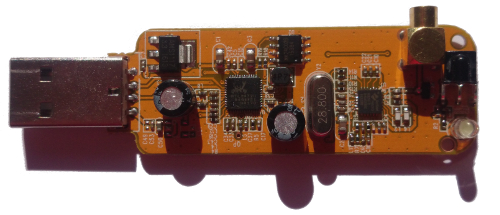
\includegraphics[width=0.5\columnwidth]{./fig/rtlsdr.jpg}
				\caption{\textit{RTL-SDR} hardware with the DVB-T I/Q
				demodulator \textit{Raeltek RTL2832U} (left IC) and the tuner
				with integrated LNA \textit{Rafael Micro R820T/2} (right IC).} 
				\label{fig:rtl_hw}
\end{figure}
The \textit{Realtek RTL2832U} is a terrestrial digital video broadcast
(DVB-T) demodulator IC, which is the main component in a wide range of
USB-based DVB-T receiver dongles. One prominent feature of this chip is
that it allows to retrieve the raw I/Q samples via USB. This is
originally intended for the chip to work as a simple DAB/FM software
receiver. Ham radio enthusiasts have combined their efforts to create a
software driver (the \textit{librtlsdr}~\cite{steve-m_librtlsdr})
that allows DVB-T dongles based on the \textit{RTL2832} to be converted
into low-cost wideband SDR receivers. The cost of traditional SDRs is
in the range of a few hundred to thousands of USD. Albeit much less
powerful than a typical SDR, a \textit{RTL2832U}-based DVB-T receiver
can be bought with antenna for less than 10 USD.  

An RTL-SDR also contains a tuner that allows the user to select the
received frequency.  In our case the tuner is a \textit{Rafael Micro
R820T/2} which offers a tuning range from 42 to 1002
MHz~\cite{rafael_r820t_2011}. Figure \ref{fig:rtl_hw}, shows a
photograph of the RTL-SDR used in our work. 

\subsection{Quadrature Demodulation}

Quadrature demodulation is the major feature of the \textit{RTL2832U},  which makes it possible to decode a digitally amplitude- and phase-shifted signal. The received signal (behind the tuner at the input of the \textit{RTL2832U}) can be interpreted as
\begin{equation}
	s_{\text{RF}}(t)=I(t) \cdot cos(\omega_{0}t) + Q(t) \cdot sin(\omega_{0}t)
\end{equation}     
This is multiplied with a cosine of the carrier frequency from a local oscillator.
\begin{multline}
        s_{\text{RF}}(t) \cdot s_{\text{LO}}(t) = I(t) \cdot cos(\omega_{0}t) \cdot cos(\omega_{0}t)\\+ Q(t) \cdot sin(\omega_{0}t) \cdot cos(\omega_{0}t)
\end{multline}
With \ensuremath{2\,cos(a)cos(b)=cos(a-b)+cos(a+b)} and \ensuremath{2\,sin(a)cos(b)=sin(a+b)+sin(a-b)} follows
\begin{multline}
        2 \cdot s_{\text{RF}}(t) \cdot s_{\text{LO}}(t) = I(t) \cdot \bigl[1+cos(2\omega_{0}t)\bigr]\\+ Q(t) \cdot \bigl[sin(2\omega_0t)+sin(0)\bigr].
\end{multline}
One can see, that the interesting in-phase part (I) in this case is
represented by a DC value after mixing. With a low-pass filter this DC
value can be separated from the undesired rest. An analogous procedure
is done with the quadrature part (Q) when mixing with a sine.

\section{Design}
In this section, we describe the design 
of our system. We first describe the
design of the transmitter, next we describe 
the design of the receiver.

\subsection{Transmitter}
 
We design our backscatter transmitter to be used with ambient
television signals.  We design the transmitter for ambient
television signal present in the band with  
center frequency of \SI{626}{\mega\hertz}. Crucial to the design
of the transmitter is the implementation of an antenna, as
the antennas are known to be  frequency selective. To this end, we design an
antenna on an unetched board made of FR4 substrate commonly
used to design PCBs. The board acts like the ground plane, at the center
of the board we have a wire acting as a monopole antenna element. 
The antenna has a quite good reflection coefficient \ensuremath{S_{11}} 
of -17 dB at 626 MHz, which is the frequency aimed for. This means, that at 
this frequency the antenna absorber more energy form the electromagnetic field compared to another band. A vector network analyzer (VNA) has been used to analyze antenna performance.

Backscatter operates by reflecting or absorbing impinging
radio signals on the antenna. To purposefully toggle the antenna
to achieve these states, we  terminate the antenna to a 
RF switch. The RF switch enables us to alternate the impedance connected to
the antenna between matched (50 \ensuremath{\Omega}) and open state.
We control the RF switch through an I/O pin on a low-powered MCU, Texas
instruments MSP430. As discussed earlier, to reduce the effects of
self-interference, we frequency-shift the backscatter transmission
away from the TV signal. Hence, we operate the RF switch using a 
\SI{2}{\mega\hertz} intermediate frequency signal. Therefore the result 
is a frequency shift of the television signal by 2 MHz, when
transmitting a bit 1, and no shift for a 0.  Hence,  we 
leverage amplitude modulation at receiver in our design.
 
\subsection{Receiver}
\begin{figure}[h]
\centering
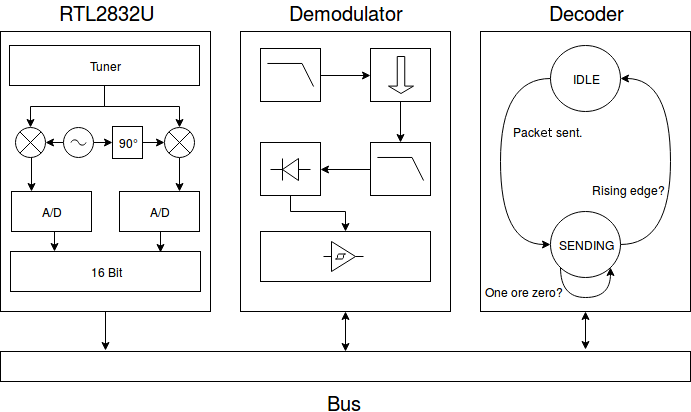
\includegraphics[width=\columnwidth]{./fig/receiver_arch}
\vspace{-6mm}
\caption{\emph{Design of the ambient backscatter receiver.} The flow of operation of the
receiver is from the left to right.}
\label{fig:receiver_arch}
\vspace{-6mm}
\end{figure}
The receiver consists of three main modules interconnected by a bus. The
RTL-SDR block is in charge of collecting samples from the SDR-device. The
demodulator turns the sampled signal into a streams of ones and zeroes.
Finally, the Decoder block is in charge of detecting frames. We provide our C++
receiver code publicly available under~\cite{s3xm3x_backscatterBASKReceiver}.

%A highly
%sophisticated bus system has been developed to exchange data between the
%different components of the system. 
Figure \ref{fig:receiver_arch} shows the architecture of our receiver, the
signal flows from the left to the right.
%\textit{Librtlsdr} (cf. \cite{steve-m_librtlsdr}), which is based on
%\textit{libusb}, is used to transfer the data from the TV stick into our
%program. As described in section~\ref{sub:rtl2832}, the RTL2832 mixes
%down the high frequency to a intermediate frequency (both values are
%software adjustable). Subsequently the data is mixed with sine and
%cosine, low-pass filtered and finally transferred to the digital domain.
The raw I/Q data is available as two 8-bit values (real and imaginary) from the
RTL-SDR. With these two values, the phase and magnitude of the data can be
determined for every sample. The received signal can be represented as:
\begin{equation}
	I+j\,Q = abs(I,Q) \cdot e^{j \cdot ang(I,Q)} 
\end{equation} 
 
So the first block, entitled RTL2832U, provides the interface to the TV
dongle. It controls the frequency \ensuremath{f_{tuned}}, where the
receiver is listening as well as other interesting parameters e.g. the analog gain.

The demodulator block is responsible for converting the sampled signals
into ones and zeroes. 
As part of the demodulation process the signal is down-sampled and
low-pass-filtered two times. The last demodulation step is to rectify
the signal (cf. equation \ref{eq:rectify}) and decide with a
software-defined Schmitt trigger whether a sample is a 1 or a 0.  
\begin{equation}
	\label{eq:rectify}
	abs(I,Q) = \sqrt{I^2 +  Q^2}
\end{equation} 

The resulting values are sent through the bus to the decoder. After the decoder
received the samples it decides if a frame is received or if the channel is
idle. The decoder also includes a function to correlate the received bitstream
with an expected pattern. Hence it is able to determine the bit error ratio
(BER). Furthermore we have implemented a series of aditional tools that include
different simulators for e.g. playing back recorded data and a tool (an
oscilloscope) to plot the data, which is written into files by the demodulator.
An example of a recorded data stream with 25 kS/s can be seen in Figure
\ref{fig:transmission}.  


\begin{figure}[h]
\centering
\vspace{-30mm}

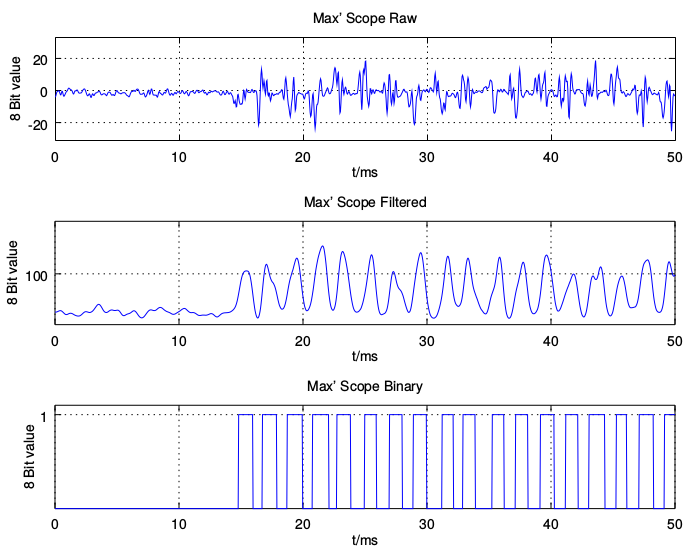
\includegraphics[width=\columnwidth]{./fig/transmission}
\vspace{-30mm}
\caption{Data from the Octave oscilloscope showing the start of a transmission of 101010.. with 1 kbit/s with idle state before. The amplitude is quite low with an average of 12 \% of the maximum, which is 127.5. This is due to a low signal strength. Sampling frequency is 25 kHz. At the top one can see the raw signal from the ADC, in the middle the filtered signal and at the bottom the signal after the Schmitt trigger.}
\label{fig:transmission}
\vspace{-6mm}

\end{figure}

\section{Evaluation}

In this section, we present the results of evaluation of our system. As experimental 
setup, we use RTL-SDR together with a signal processing algorithm implemented
in Octave. 

\subsection{Spatial variation of ambient television signals}

\begin{figure}[h]
	\centering
	\begin{minipage}{0.49\columnwidth}
	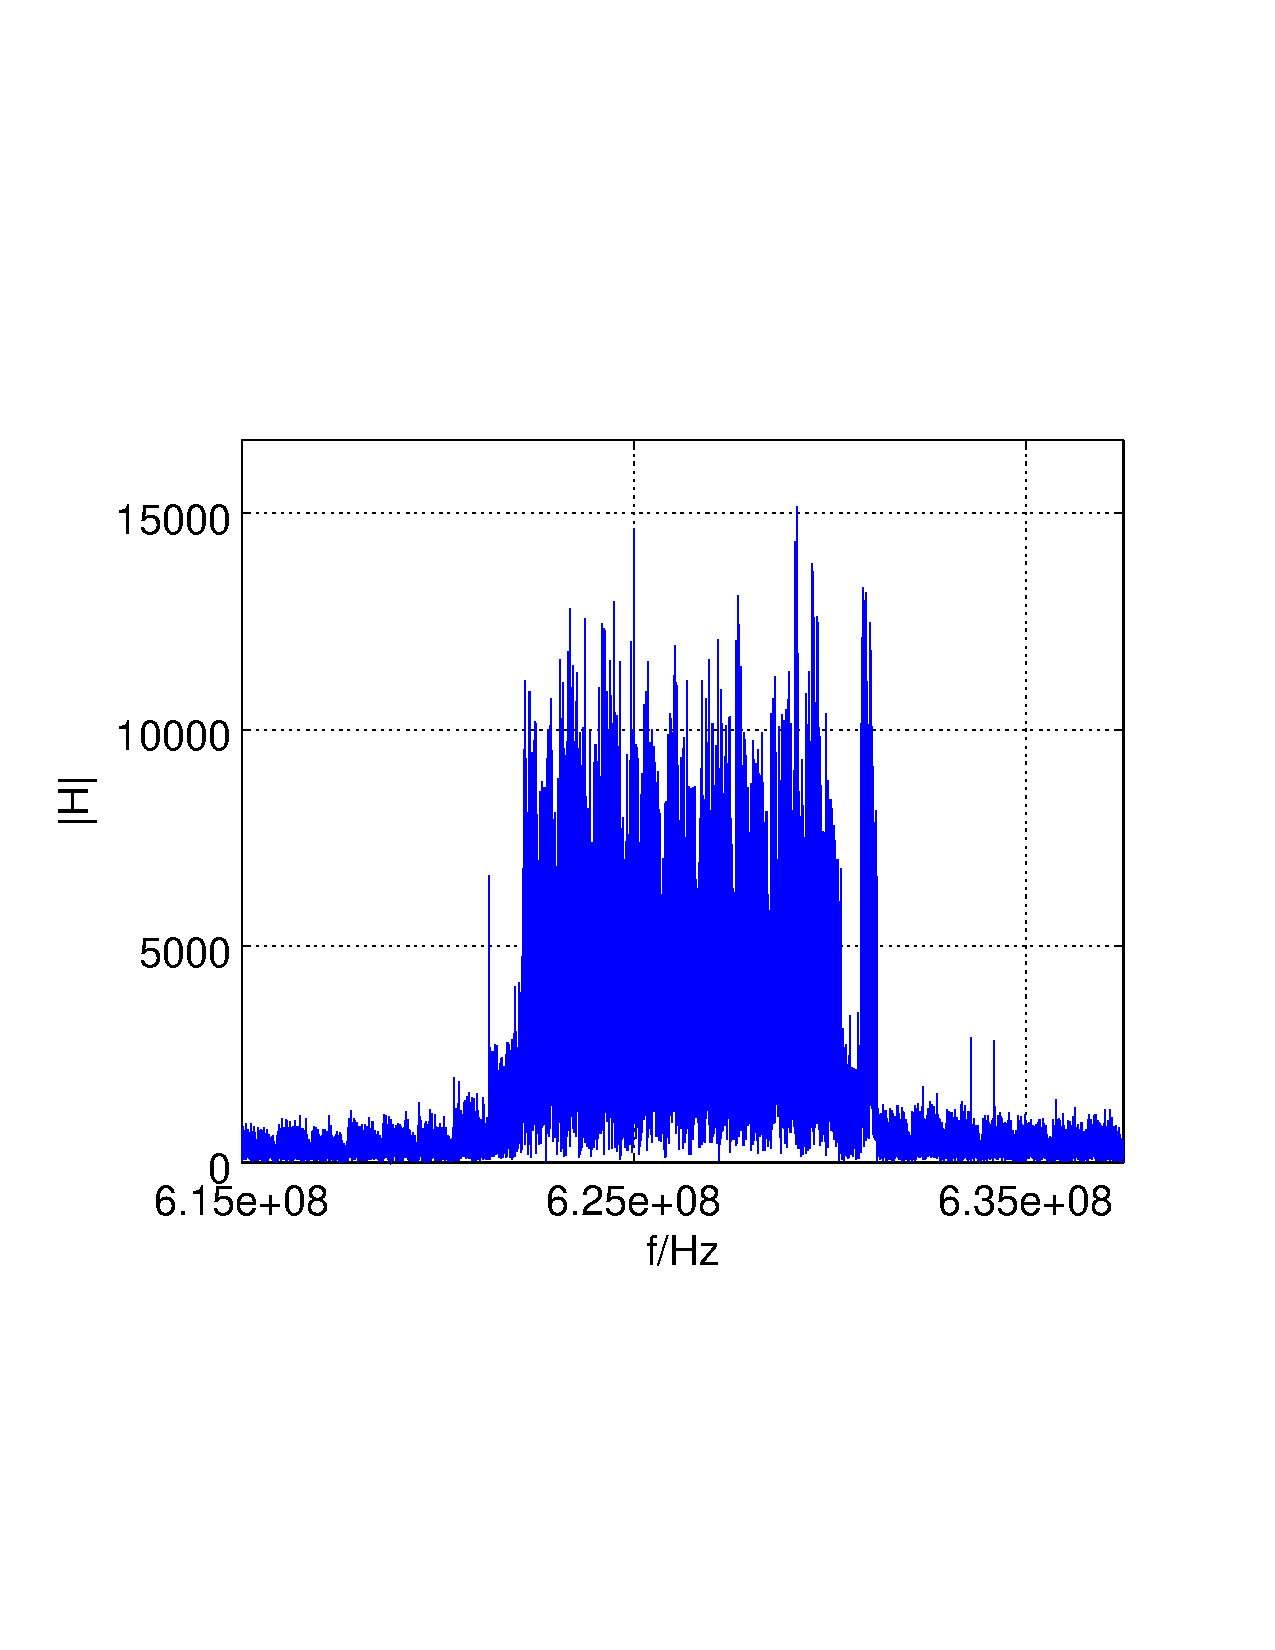
\includegraphics[width=\columnwidth]{./fig/626mhz_raw}
	\end{minipage}
	\hfill
	\begin{minipage}{0.49\columnwidth}
	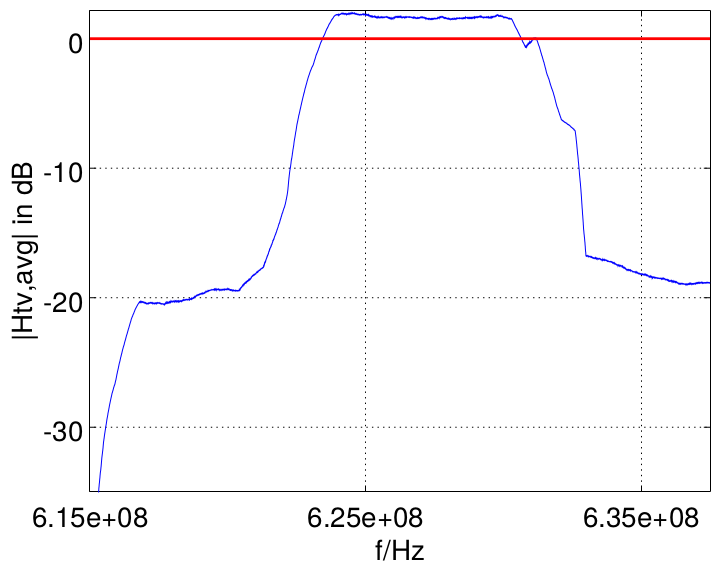
\includegraphics[width=\columnwidth]{./fig/626mhz_filtered}
	\end{minipage}
	\vspace{-6mm}
	\caption{\emph{Observed spectrum of television signal}. The left hand image shows the raw spectrum of the TV signal, with centre frequency of \SI{626}{\mega\hertz}. The right hand image shows the smoothed spectrum normalized to maximum average. The average is  shown by the horizontal red line.}
	\label{fig:tv_record} 
		\vspace{-6mm}
\end{figure}

In this experiment, we investigate the variation of the television signal
in space, i.e., how does the strength of the signal varies over 
the area of the city. We use the RTL-SDR reader to obsevre the signal strength.
We perform the frequency sweep of the desired television band. Next, we
obtain the sample in the time domain, and convert them to corresponding
samples in frequency domain by performing fast-fourier transformation~(FFT).

As we are not interested in realtime visualisation of the television
signals, we acquire the signals offline and visualise the samples.
RTL-SDR has a maximum sampling rate of 2.4 MS/s, which limits us to
scanning a band of \SI{1.2}{\mega\hertz} band in a single run. We  keep some safety-margin, and
sample the desired band at \SI{900}{\kilo\hertz} intervals. We sample the band 
\SI{20}{\mega\hertz} wide, by stitching individual bands. In our experiments, it takes roughly 30
seconds for us to perform the scanning operation.


%These scripts are available under \cite{s3xm3x_RTLSDRSpecAn}
 
During the scanning process the gain is set to 40.2 dB. To get the
signal strength we simply take the average over a 10 MHz band around the
center frequency of the desired TV signal. This approach can be
justified by the fact, that DVB-T 2 is specified up to 10 MHz bandwidth.
And the local TV provider advertises to be transmitting DVB-T 2.
The signal \ensuremath{|H|} is calculated as follows.  
\begin{equation}
	|H| = \Biggl| \sum_{n=0}^N FFT\biggl( \Re\{ s_{\text{band,n}}(t) \} \biggr) \Biggr|
\end{equation}     where \ensuremath{N} is the total number of intervals
accumulated over the entire frequency sweep. The FFT is only carried out over
the real values, which are received from the \textit{RTL-SDR}.
\ensuremath{s_{\text{band,n}}(t)} is the signal in the time domain of one
interval (one subband). There are as many samples taken in one band as needed
for an FFT of size 2048. To finally get \ensuremath{|H_{tv,avg}|} one has to
normalize everything and calculate the power. Before doing that, a simple
smoothing algorithm (FIR) is applied on \ensuremath{|H|}.  
\begin{equation}
	|H_{\text{tv,avg}}| = 20 \cdot log (|H|) - 20 \cdot log(|H_0|)
\end{equation}   
where \ensuremath{|H_0|} is a normalization value measured at a certain point
in space. 

Figure~\ref{fig:haversine} demonstrates the result of combing the measured
signal strength values, together with the haversine function enables us to
calculate the distance from the point where the maximum signal has been
captured. The fast fading of the signal has been proven to be highly fluctuating, but it is still hight enough to enable backscattering.    

\begin{figure}[h]
	\centering
	\begin{minipage}{0.49\columnwidth}
	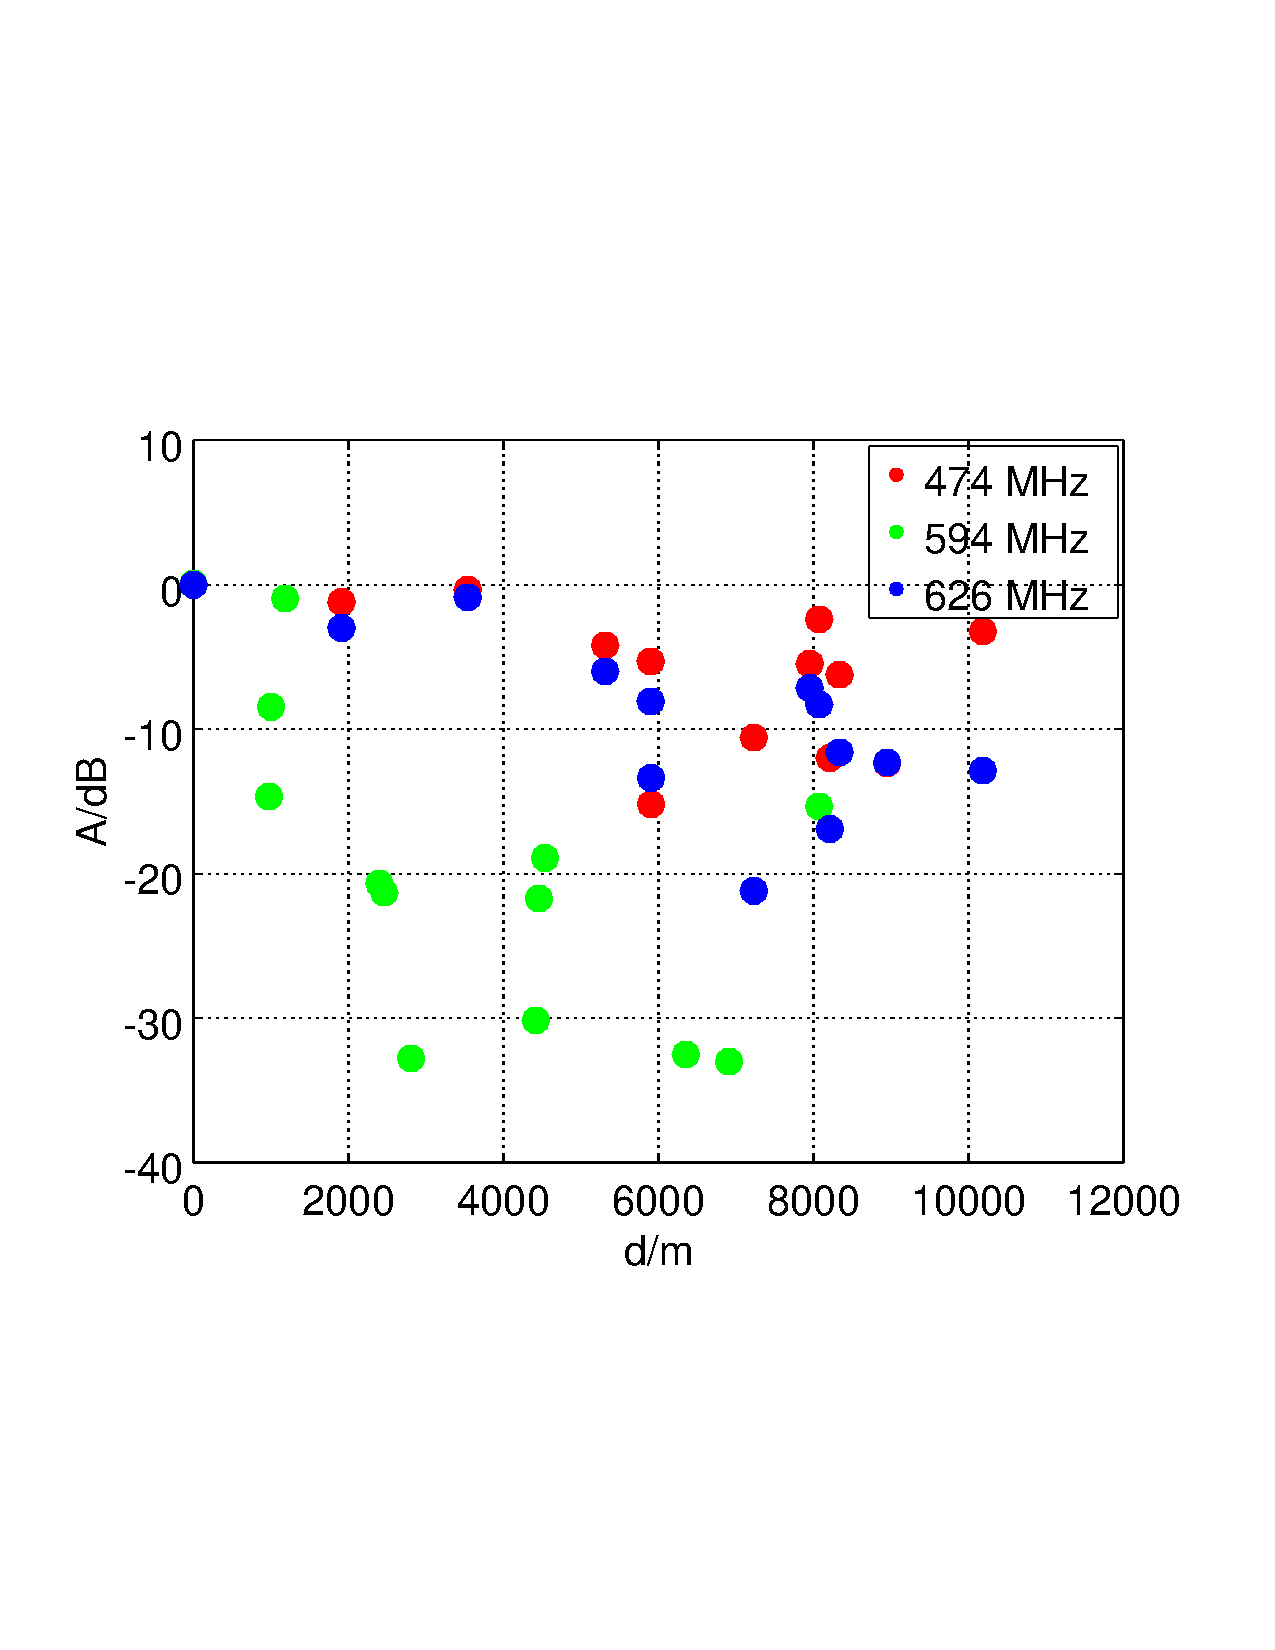
\includegraphics[width=\columnwidth]{./fig/haversine}
	\end{minipage}
	\hfill
	\begin{minipage}{0.49\columnwidth}
	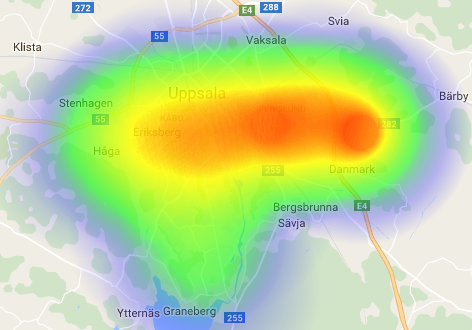
\includegraphics[width=\columnwidth]{./fig/heatmap_626mhz}
	\end{minipage}
	\vspace{-6mm}
	\caption{\emph{Spatial variation of TV signals in Uppsala city}. 
	The left image demonstrates the signal strength of TV signal fading	
	as opposed to observed signal strength near the TV tower. 
	The right image visualises the signal strength as heatmap for the signal
	present in the \SI{626}{\mega\hertz} band. Distances have been
calculated with the Haversine formula. }
 	\vspace{-6mm}

\label{fig:haversine}
\end{figure}

\balance

\subsection{Communication Performance}
In this experiment, we present some preliminary results to evaluate the communication
performance of our system.  In the experiment, we varied the bitrate of the transmitter
from 1 bit/s up to 1 kbit/s. As we had seen earlier in the Figure~\ref{fig:transmission}, the strength
of the backscattered signal is rather low leading to the appearance of significant quantisation noise.
The experiments have been carried out with the maximum gain available from the tuner of \SI{50}{\decibel}.

In an indoor environment, where the ambient signal strength is low, we are
able to achieve a data rate of 1 b/s with distances of
couple of meters. At higher bitrates, we observe a range of a few decimeters and the  bit error rate is still approximately 40 \%. 
We observed similar results outdoors. We acknowledge the high bit errors
observed due to primarily limited gain available on the low cost dongles.
In future, we will work to improve this. We note, existing ambient backscatter
systems do not operate well indoors at large distances, and our results
provide preliminary results of  improvements possible by leveraging low-cost
SDRs.


\section{Discussion}

Our system still has a lot of room for improvement.  Different
backscattering antennas could be tried to find the one with the best
combination of gain, tuning frequency and bandwidth. Moreover the
standard \textit{RTL-SDR} antenna and its coaxial cable are of low
quality.  Hence a custom antenna would be beneficial. Furthermore some
fine tuning can be made when it comes to the filter coefficients of the
different filters in the demodulator chain. Finally  errors can be
further reduced by using one of many available forward error correcting
codes.

%To come to a conclusion one can say, that 
We have shown, that
spectrum scanning over a wide band with sweeping is possible using the
\textit{RTL-SDR}.  This allowed us to perform a survey of the TV signal
strength in the city. We found that the signal strength around most of the city
is adequate for backscatter communication using our receiver. And finally we
have shown for the first time, that backscatter communication is possible with
the \textit{RTL-SDR}.

\bibliographystyle{abbrv}
\bibliography{paper}

\end{document}



